\documentclass[11pt]{beamer}
% \usetheme{Boadilla}
  \usetheme{default}


% acronyms for text or math mode
\newcommand {\ccast} {\mbox{\small CCAST}}
\newcommand {\cris} {\mbox{\small CrIS}}

\newcommand {\airs} {\mbox{\small AIRS}}
\newcommand {\iasi} {\mbox{\small IASI}}
\newcommand {\idps} {\mbox{\small IDPS}}
\newcommand {\nasa} {\mbox{\small NASA}}
\newcommand {\noaa} {\mbox{\small NOAA}}
\newcommand {\nstar} {\mbox{\small STAR}}
\newcommand {\umbc} {\mbox{\small UMBC}}
\newcommand {\uw}   {\mbox{\small UW}}

\newcommand {\fft}  {\mbox{\small FFT}}
\newcommand {\ifft} {\mbox{\small IFFT}}
\newcommand {\fir}  {\mbox{\small FIR}}
\newcommand {\fov}  {\mbox{\small FOV}}
\newcommand {\for}  {\mbox{\small FOR}}
\newcommand {\ict}  {\mbox{\small ICT}}
\newcommand {\ils}  {\mbox{\small ILS}}
\newcommand {\igm}  {\mbox{\small IGM}}
\newcommand {\opd}  {\mbox{\small OPD}}
\newcommand {\rms}  {\mbox{\small RMS}}
\newcommand {\zpd}  {\mbox{\small ZPD}}
\newcommand {\ppm}  {\mbox{\small PPM}}
\newcommand {\srf}  {\mbox{\small SRF}}
\newcommand {\sdr}  {\mbox{\small SDR}}

\newcommand {\ES} {\mbox{\small ES}}
\newcommand {\SP} {\mbox{\small SP}}
\newcommand {\IT} {\mbox{\small IT}}
\newcommand {\SA} {\mbox{\small SA}}

\newcommand {\ET} {\mbox{\small ET}}
\newcommand {\FT} {\mbox{\small FT}}

% abbreviations, mainly for math mode
\newcommand {\real} {\mbox{real}}
\newcommand {\imag} {\mbox{imag}}
\newcommand {\atan} {\mbox{atan}}
\newcommand {\obs}  {\mbox{obs}}
\newcommand {\calc} {\mbox{calc}}
\newcommand {\sinc} {\mbox{sinc}}
\newcommand {\psinc} {\mbox{psinc}}
\newcommand {\std} {\mbox{std}}

% symbols, for math mode only
\newcommand {\wnum} {\mbox{cm$^{-1}$}}
\newcommand {\lmax} {L_{\mbox{\tiny max}}}
\newcommand {\vmax} {V_{\mbox{\tiny max}}}

\newcommand {\tauobs} {\tau_{\mbox{\tiny obs}}}
\newcommand {\taucal} {\tau_{\mbox{\tiny calc}}}
\newcommand {\Vdc}  {V_{\mbox{\tiny DC}}}

\newcommand {\rIT} {r_{\mbox{\tiny\textsc{ict}}}}
\newcommand {\rES} {r_{\mbox{\tiny\textsc{es}}}}
\newcommand {\robs} {r_{\mbox{\tiny obs}}}

\newcommand {\rITobs} {r_{\mbox{\tiny\textsc{ict}}}^{\mbox{\tiny obs}}}
\newcommand {\rITcal} {r_{\mbox{\tiny\textsc{ict}}}^{\mbox{\tiny cal}}}

\newcommand {\ITmean} {\langle\mbox{\small IT}\rangle}
\newcommand {\SPmean} {\langle\mbox{\small SP}\rangle}


\title{new cris calibration \\ 
       algorithm comparisons
}
\author{H.~E.~Motteler, L.~L.~Strow}
\institute{
  UMBC Atmospheric Spectroscopy Lab \\
  Joint Center for Earth Systems Technology \\
}
\date{\today}
\begin{document}

%----------- slide --------------------------------------------------%
\begin{frame}[plain]
\titlepage
\end{frame}
%----------- slide --------------------------------------------------%
\begin{frame}
\frametitle{introduction}

\begin{itemize}

  \item we compare an updated version of {\ccast} with our
    implementation of \noaa~4.  This allows for identical \ils,
    translation to the user grid, and other processing details,
    so the only difference is the calibration equation

  \item we show results for both clear matchups and \fov~5 relative
    tests, including tests of both algorithms with and without
    responsivity

  \item after reviewing the 10 June 2015 calibration algorithm
    comparisons of Yong Han and Yong Chen, we modified the {\ccast}
    processing filters to be closer to the new \noaa\ filters

  \item the \ccast\ filters can not be identical because the
    ratio-first algorithm needs to roll off the calibration ratio
    inside instrument responsivity

\end{itemize}

\end{frame}
%----------- slide --------------------------------------------------%
\begin{frame}
\frametitle{methods}

\begin{itemize}

  \item for tests with calculated radiance we start with 2300 
    clear matchups from ccast granule SDR\_d20150218\_t0318115 and
    calculate upwelling radiances with kcarta at a 0.0025 cm-1 grid

  \item for the ``flat'' tests the new ccast processing filters are
    applied pointwise and the result is convolved to the {\cris}
    user grid

  \item for the ``resp'' tests instrument responsivity is applied
    pointwise to the kcarta radiances, these are convolved to the
    user grid, and then divided pointwise by inverse responsivity

  \item relative tests are with data averaged over the three day
    test period, 17-19 Feb 2015
    
  \item all test are done with periodic sinc wrapping at the sensor
    grid, added guard points, and double Fourier interpolation to
    the user grid

\end{itemize}

\end{frame}
%----------- slide --------------------------------------------------%
\begin{frame}
\frametitle{ccast and noaa LW filters}
\begin{center}
  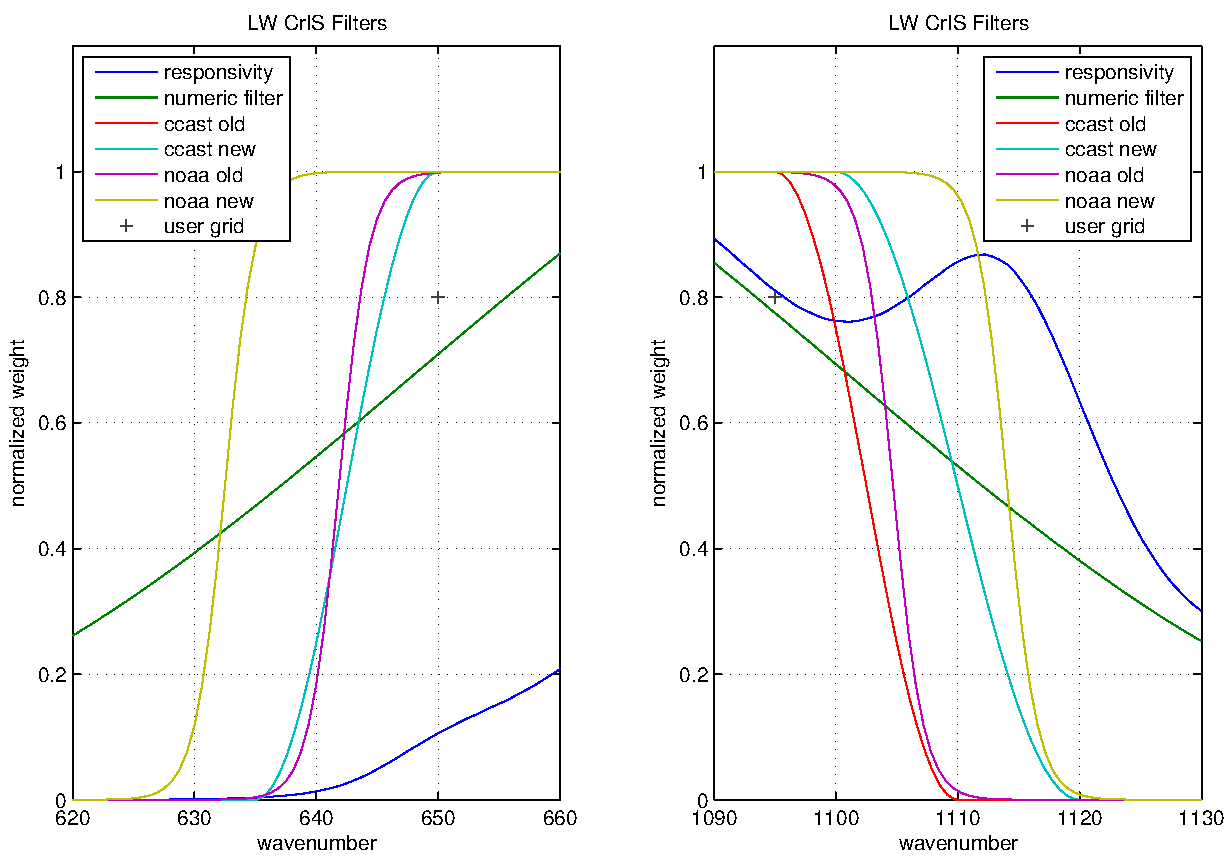
\includegraphics[scale=0.5]{figures/show_filts_LW.pdf}
\end{center}
\end{frame}
%----------- slide --------------------------------------------------%
\begin{frame}
\frametitle{ccast and noaa MW filters}
\begin{center}
  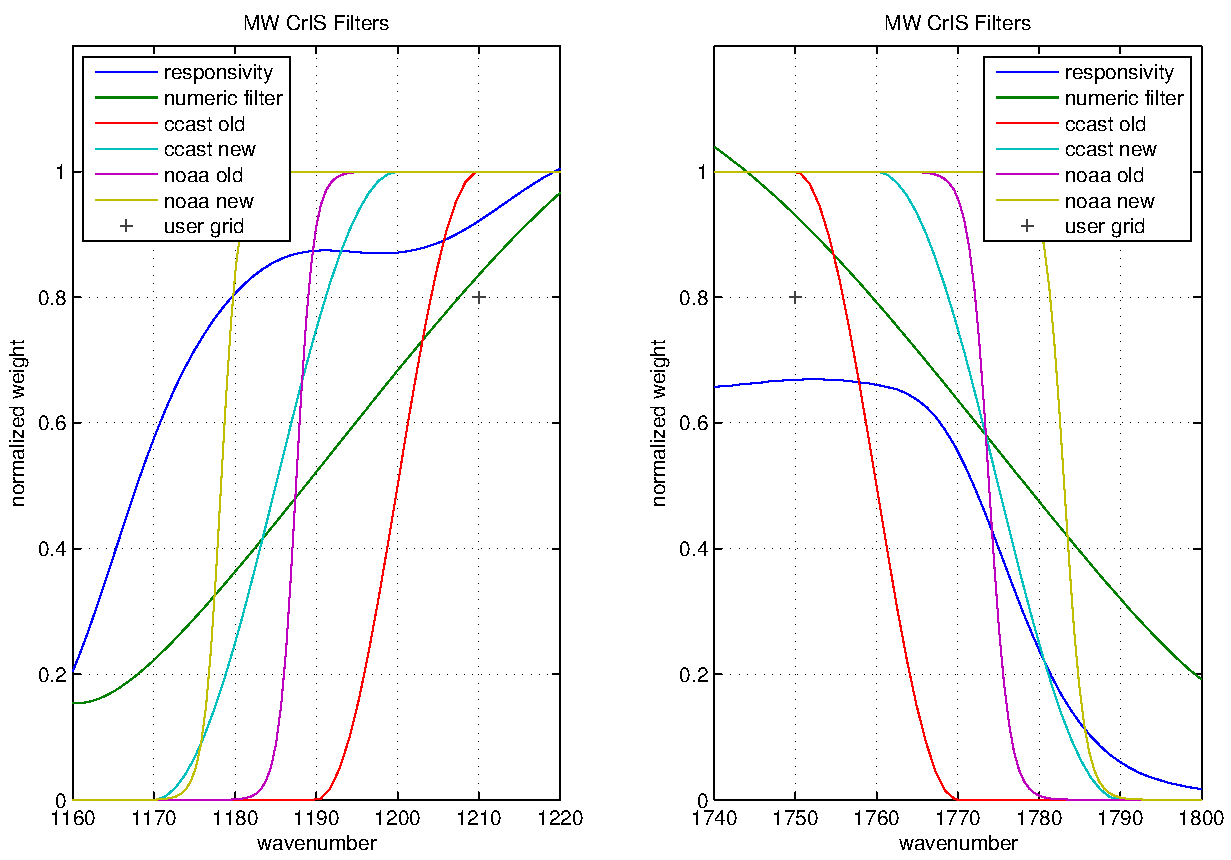
\includegraphics[scale=0.5]{figures/show_filts_MW.pdf}
\end{center}
\end{frame}
%----------- slide --------------------------------------------------%
\begin{frame}
\frametitle{ccast and noaa SW filters}
\begin{center}
  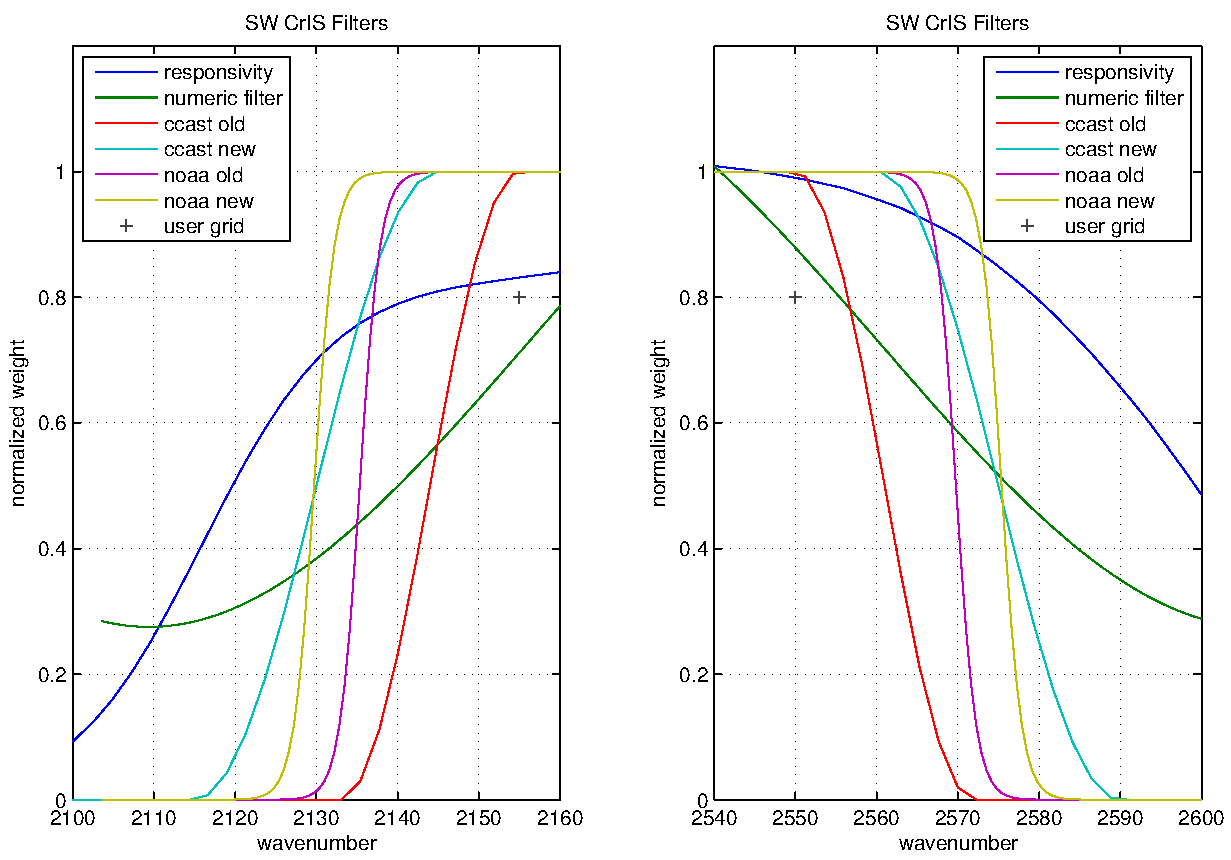
\includegraphics[scale=0.5]{figures/show_filts_SW.pdf}
\end{center}
\end{frame}
%----------- slide --------------------------------------------------%
\begin{frame}
\frametitle{responsivity vs flat reference truth}
\begin{center}
  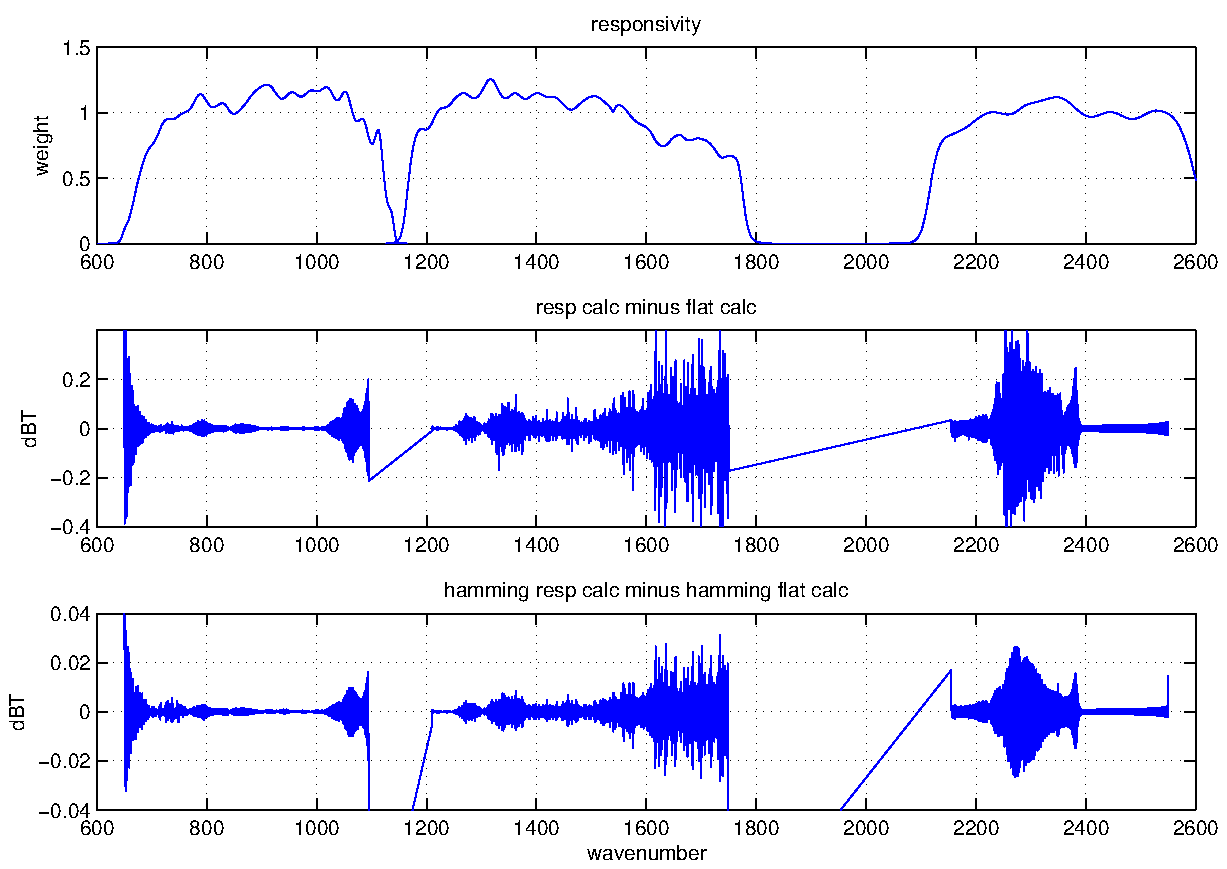
\includegraphics[scale=0.5]{figures/resp_flat_diff.pdf}
\end{center}
\end{frame}
%----------- slide --------------------------------------------------%
\begin{frame}
\frametitle{obs minus calc overview}
\begin{center}
  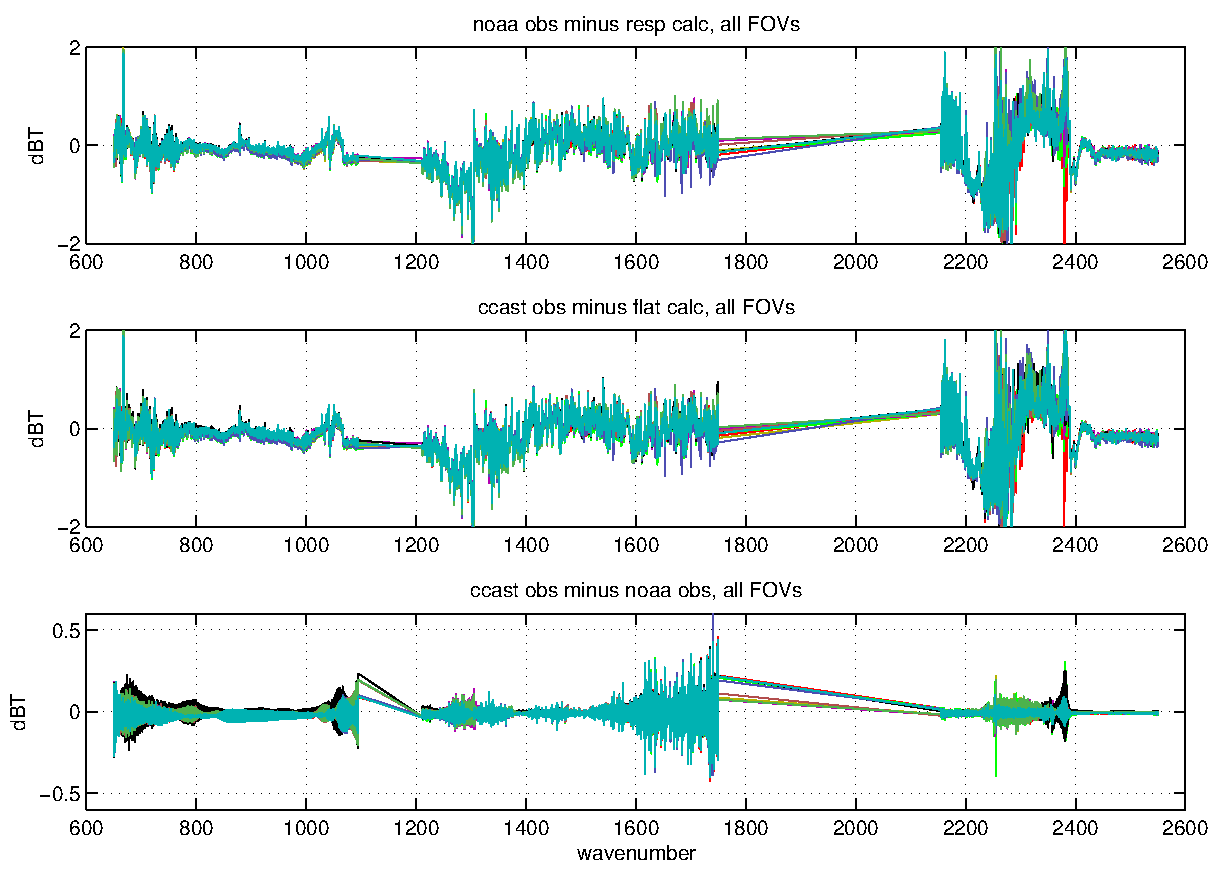
\includegraphics[scale=0.5]{figures/cal_summary.pdf}
\end{center}
\end{frame}
%----------- slide --------------------------------------------------%
\begin{frame}
\frametitle{obs minus calc LW detail}
\begin{center}
  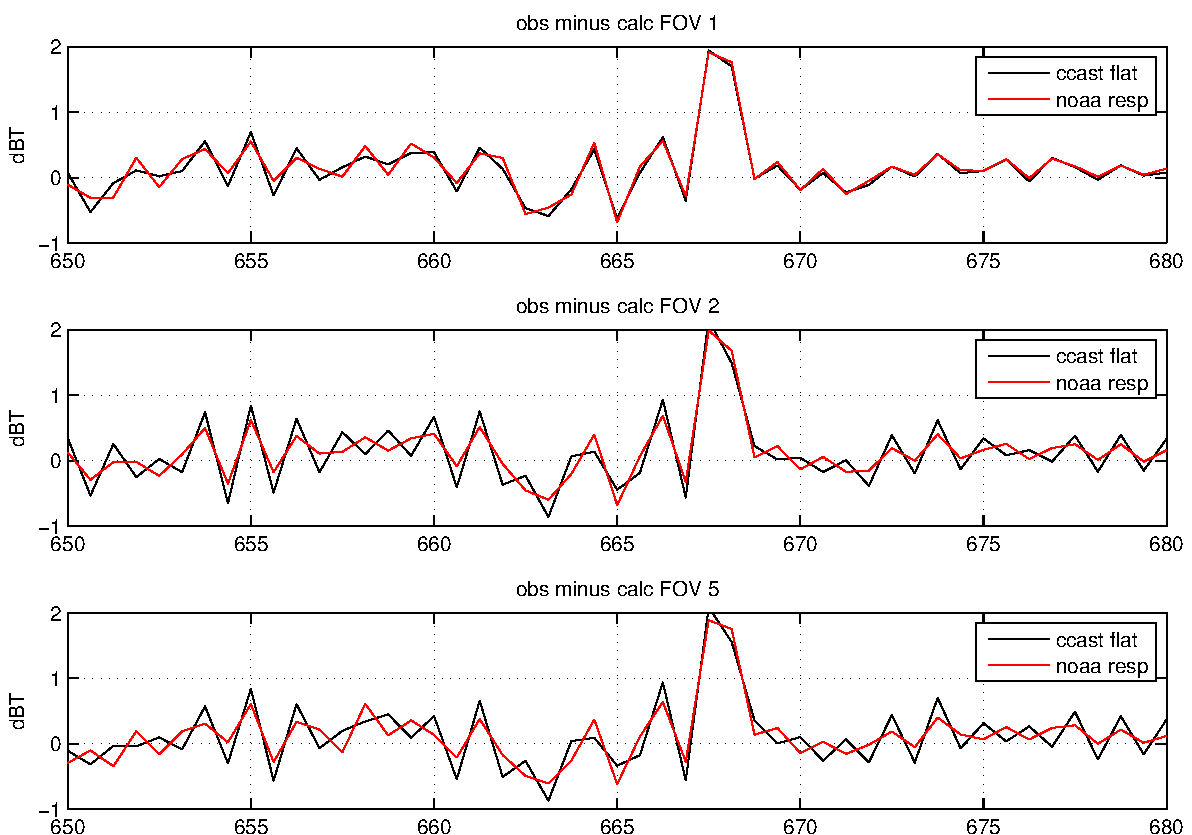
\includegraphics[scale=0.5]{figures/cal_LW_detail.pdf}
\end{center}
\end{frame}
%----------- slide --------------------------------------------------%
\begin{frame}
\frametitle{noaa all fovs LW detail}
\begin{center}
  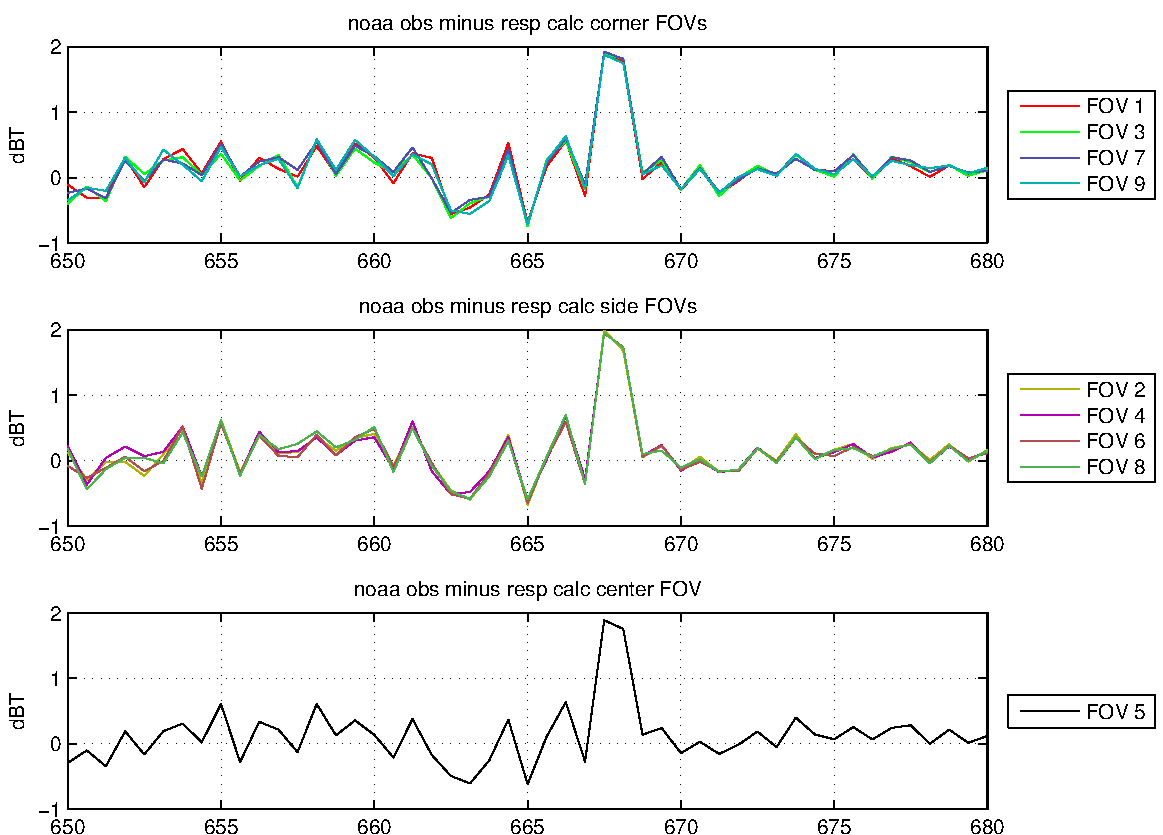
\includegraphics[scale=0.5]{figures/cal_noaa_LW.pdf}
\end{center}
\end{frame}
%----------- slide --------------------------------------------------%
\begin{frame}
\frametitle{ccast all fovs LW detail}
\begin{center}
  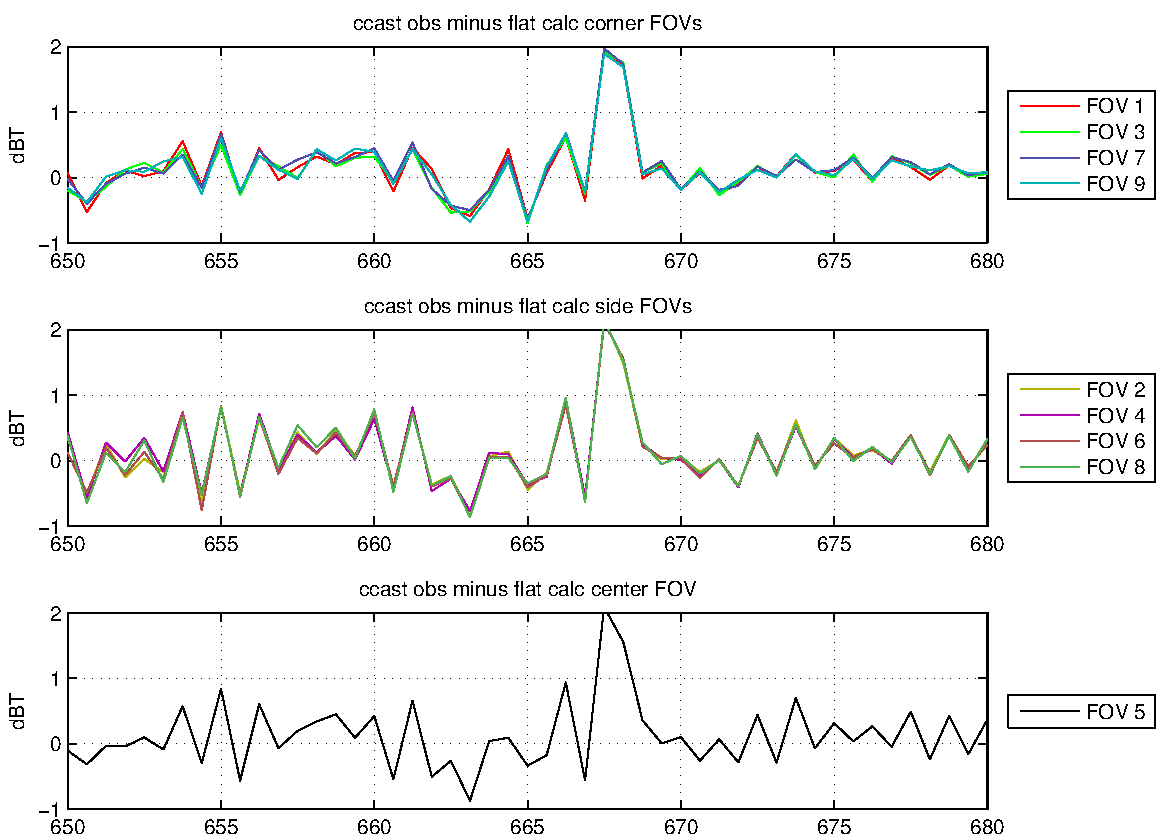
\includegraphics[scale=0.5]{figures/cal_ccast_LW.pdf}
\end{center}
\end{frame}
%----------- slide --------------------------------------------------%
\begin{frame}
\frametitle{obs minus calc MW detail}
\begin{center}
  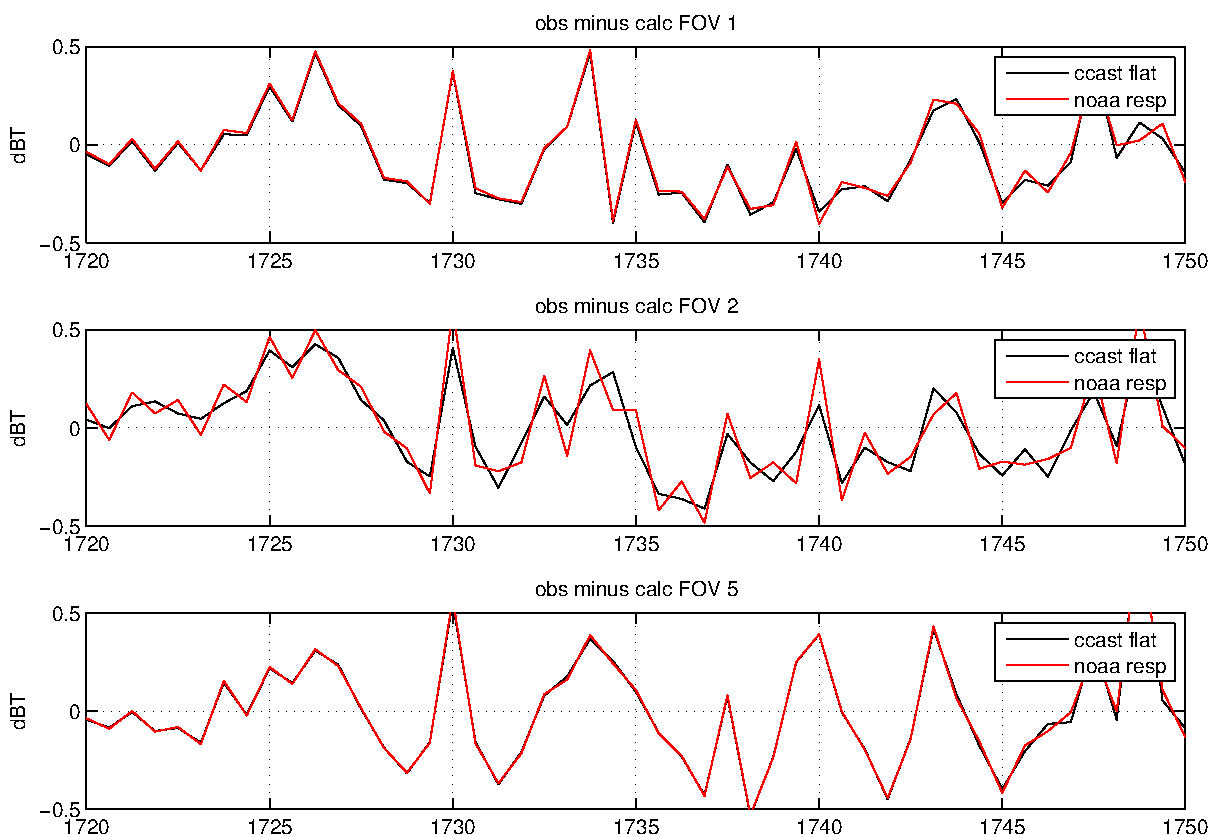
\includegraphics[scale=0.5]{figures/cal_MW_detail.pdf}
\end{center}
\end{frame}
%----------- slide --------------------------------------------------%
\begin{frame}
\frametitle{noaa all fovs MW detail}
\begin{center}
  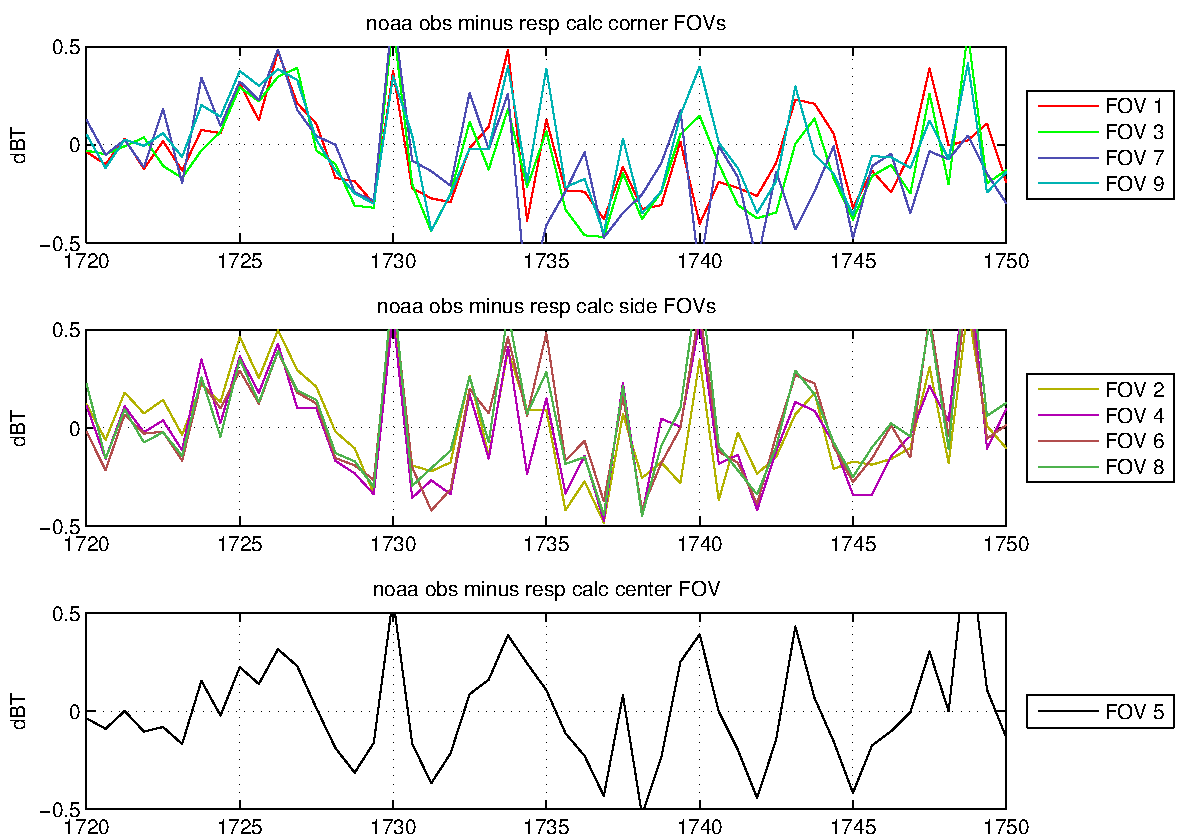
\includegraphics[scale=0.5]{figures/cal_noaa_MW.pdf}
\end{center}
\end{frame}
%----------- slide --------------------------------------------------%
\begin{frame}
\frametitle{ccast all fovs MW detail}
\begin{center}
  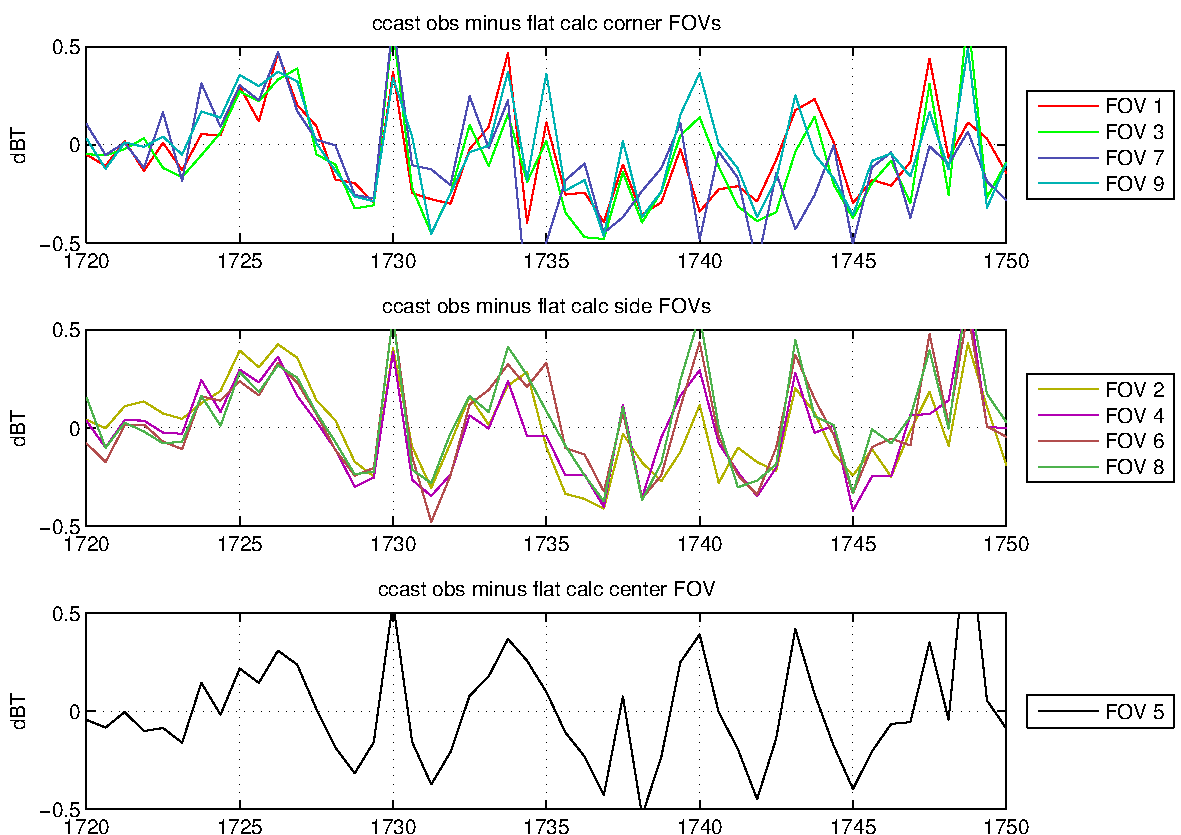
\includegraphics[scale=0.5]{figures/cal_ccast_MW.pdf}
\end{center}
\end{frame}
%----------- slide --------------------------------------------------%
\begin{frame}
\frametitle{obs minus calc summary}

\begin{itemize}

  \item at the level of detail in the overview, {\ccast} minus flat
    and {\noaa} minus resp are relatively close 

  \item the main differences are below 700 cm-1 in the LW, where
    {\ccast} is slightly worse, and above 1600 cm-1 in the MW, where
    it is slightly better

  \item in the LW detail we see \fov~1 in good agreement above
    around 665 cm-1 but {\noaa} better for \fov~2 and 5

  \item in the MW detail we see {\noaa} and {\ccast} in generally
    good agreement for \fov~5,  {\ccast} slightly better for \fov~1, 
    and significantly better for \fov~2

  \item the breakouts by FOV show both {\noaa} and {\ccast} with
    distinct side and corner FOV groups, and results generally as
    noted above

\end{itemize}

\end{frame}
%----------- slide --------------------------------------------------%
\begin{frame}
\frametitle{noaa resp and ccast flat double diffs}
\begin{center}
  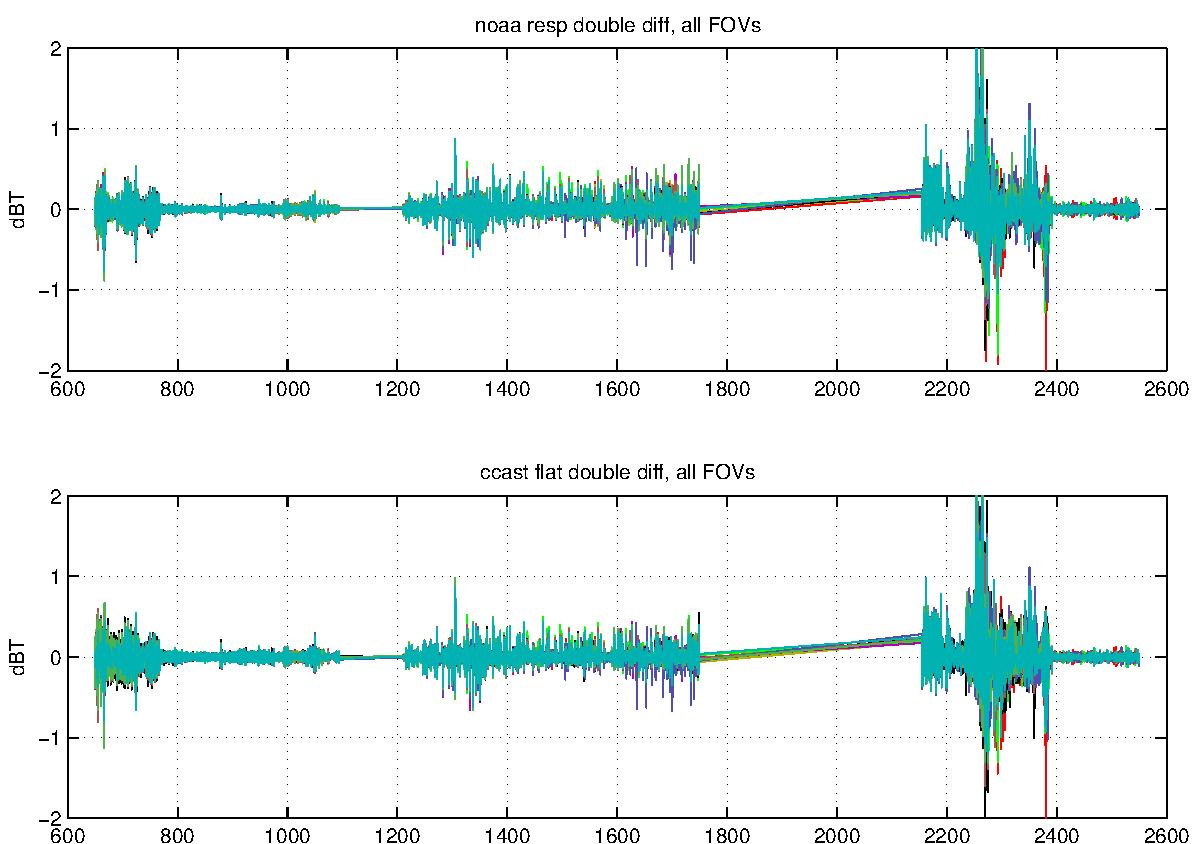
\includegraphics[scale=0.5]{figures/cal_ddif_1.pdf}
\end{center}
\end{frame}

%----------- slide --------------------------------------------------%
\begin{frame}
\frametitle{noaa flat and ccast resp double diffs}
\begin{center}
  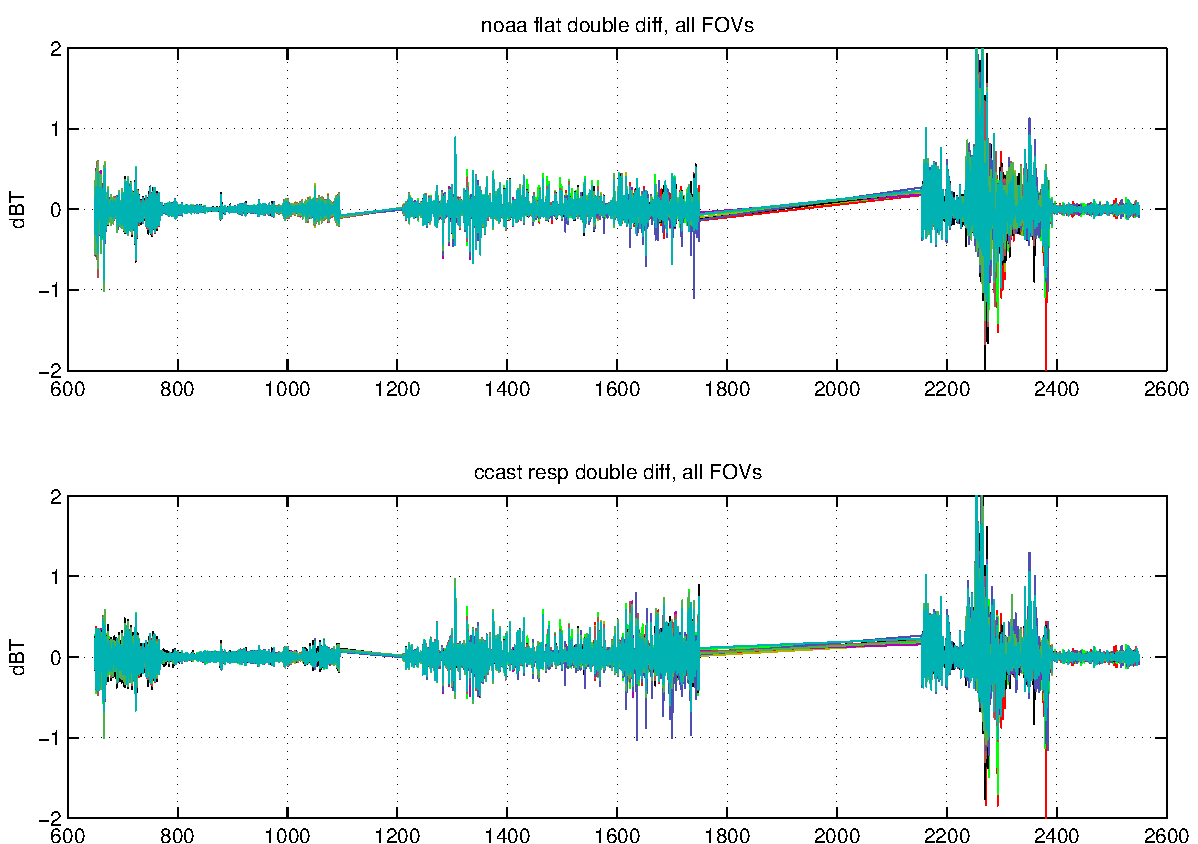
\includegraphics[scale=0.5]{figures/cal_ddif_2.pdf}
\end{center}
\end{frame}

%----------- slide --------------------------------------------------%
\begin{frame}
\frametitle{double difference summary}

\begin{itemize}

  \item the {\noaa} double difference is \[(\mbox{\small noaa obs} -
    \mbox{\small noaa resp}) - (\mbox{\small noaa apodized obs} -
    \mbox{\small noaa apodized resp})\]  
    other double differences are analogous

  \item {\noaa} with responsivity and ccast with flat reference
    truth are generally similar, with {\ccast} slightly worse at the
    low end of the LW and slightly better in MW above around 1600
    cm-1

  \item adding responsivity improves {\ccast} slightly at the low
    end of the LW and possibly in the SW, but makes it significantly
    worse above 1600 cm-1 in the MW

  \item removing responsivity generally makes {\noaa} slightly worse
    in the LW and SW, and possibly also in the MW

\end{itemize}

\end{frame}
%----------- slide --------------------------------------------------%
\begin{frame}
\frametitle{relative test overview}
\begin{center}
  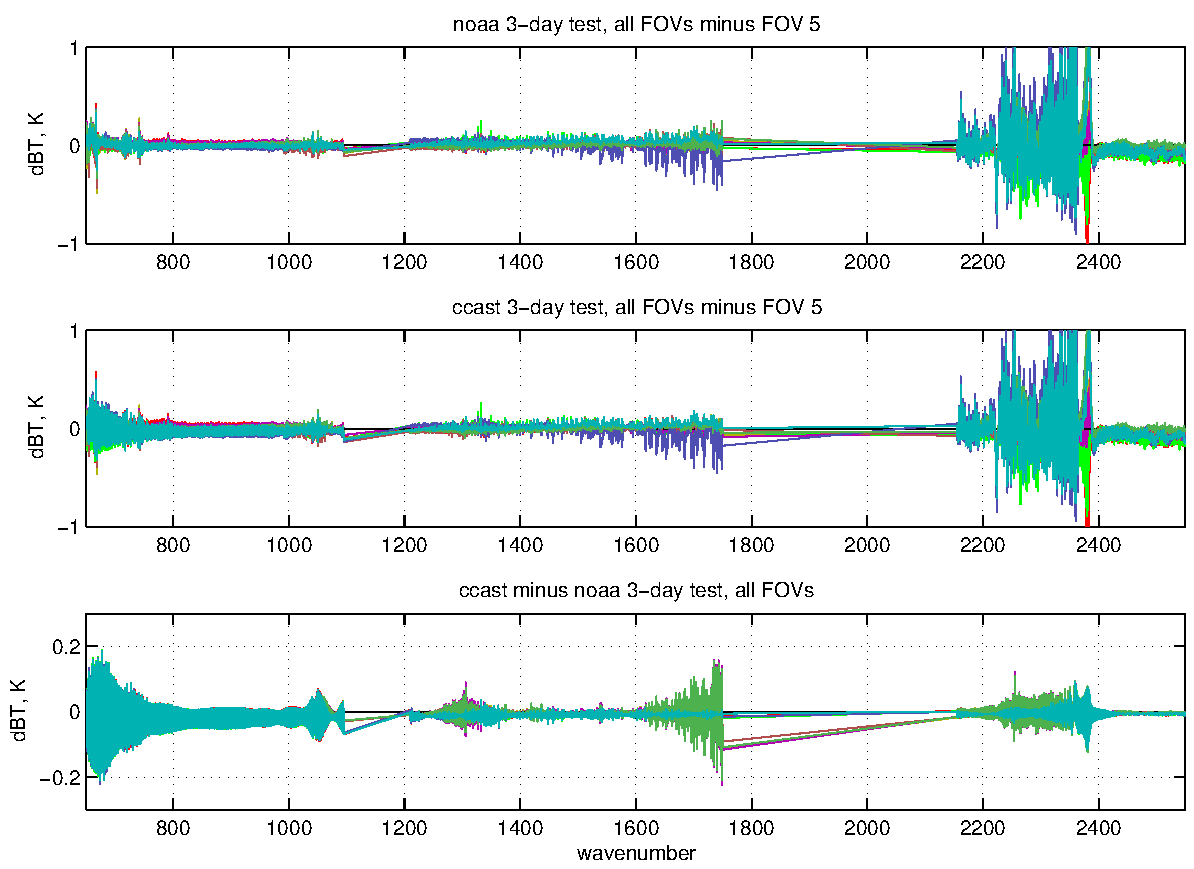
\includegraphics[scale=0.5]{figures/rel_summary.pdf}
\end{center}
\end{frame}

%----------- slide --------------------------------------------------%
\begin{frame}
\frametitle{noaa relative double diffs}
\begin{center}
  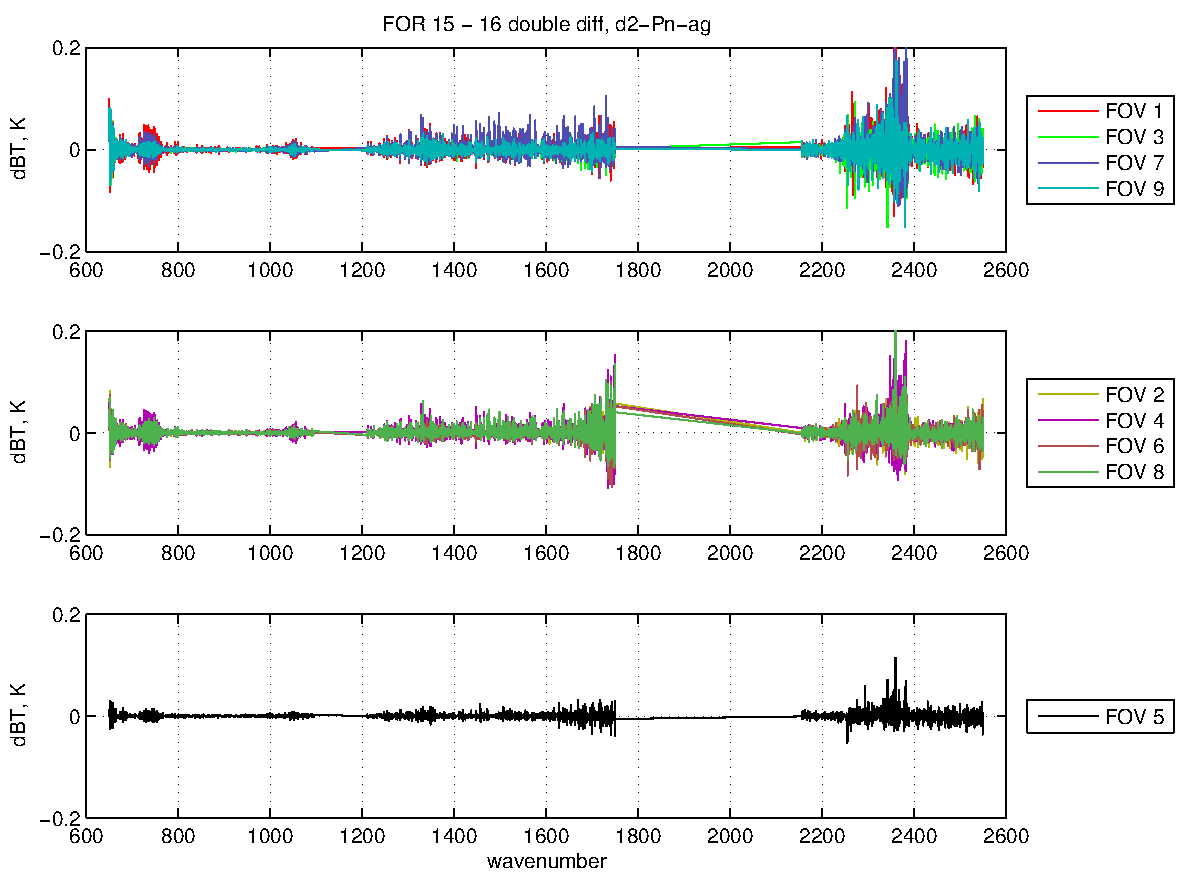
\includegraphics[scale=0.5]{figures/rel_noaa_ddif.pdf}
\end{center}
\end{frame}

%----------- slide --------------------------------------------------%
\begin{frame}
\frametitle{ccast relative double diffs}
\begin{center}
  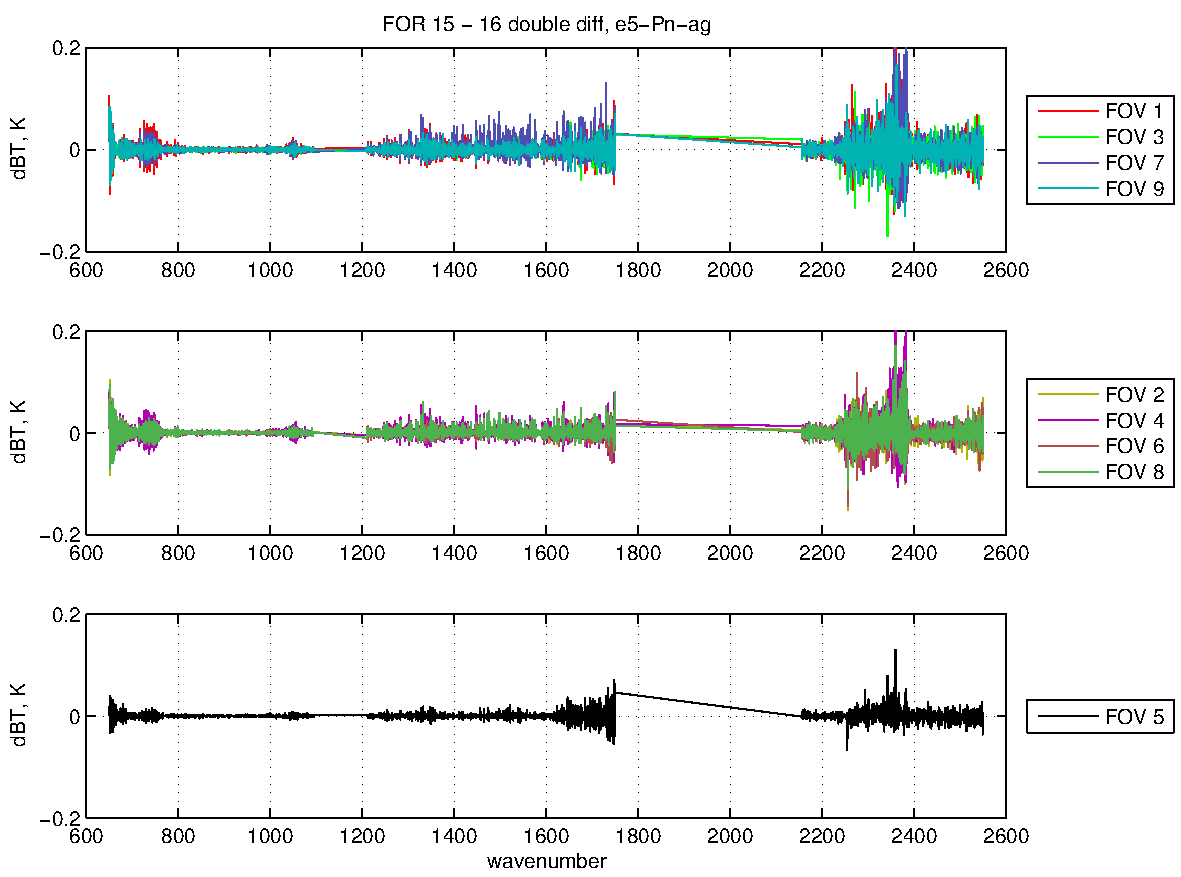
\includegraphics[scale=0.5]{figures/rel_ccast_ddif.pdf}
\end{center}
\end{frame}

%----------- slide --------------------------------------------------%
\begin{frame}
\frametitle{relative test summary}

\begin{itemize}

  \item the overview is the difference from FOV 5 of the means of
    FOR 15 and 16 taken together

  \item the double differences here are \[(\mbox{\small FOR 15} -
    \mbox{\small FOR 16}) - (\mbox{\small apodized FOR 15} -
    \mbox{\small apodized FOR 16})\]

  \item relative test results are generally consistent with the obs
    minus calc tests shown earlier

  \item {\ccast} is worse in the LW and slightly better in the MW
    above around 1600 cm-1.  Some of the LW difference may be due to
    the \fov~5 differences we saw in the obs minus calc tests

  \item the relative double differences are small in comparison with
    other residuals shown here, with {\noaa} a little better overall
    but {\ccast} significantly better for side FOVs in the MW

\end{itemize}

\end{frame}
%----------- slide --------------------------------------------------%
\begin{frame}
\frametitle{conclusions}

\begin{itemize}

  \item we have seen a significant convergence in calibration
    algorithm results and performance

  \item overall the {\noaa} algorithm works slightly better with
    responsivity and {\ccast} better without

  \item remaining differences between the {\ccast} and {\noaa}
    calibration equations are small

  \item {\ccast} flat is slightly worse at the LW end of the LW
    band, and slightly better in the MW above around 1600 cm-1

  \item differences after Hamming apodization are very small

  \item although the {\noaa} algorithm has a few more steps, this
    has no significant effect on runtime

\end{itemize}

\end{frame}
%----------- slide --------------------------------------------------%
\begin{frame}
\frametitle{context for SDR reference truth choices}

\begin{itemize}

  \item {\ccast} flat output close to true sinc \ils

  \item {\ccast} flat RTA simulation requires 3 bandpass filters \\
    (12 parameters)

  \item {\noaa} resp RTA simulation requires full responsivity curves
    (roughly 1700 parameters)


  \item {\noaa} resp radiance climate record may be affected if
    responsivity varies from instrument to instrument or changes for
    a particular instrument

  \item {\cris} flat radiances insensitive to filter characteristic

  \item LLS believe is will be hard to get international community to
    use responsivity in the long time frame!  Debatable

  \item Impact of cal eqn and reference truth choices: Later Talk

\end{itemize}

\end{frame}
%----------- slide --------------------------------------------------%
\begin{frame}
\frametitle{ccast calibration equation}

\[\rES = F \cdot \rIT \cdot f \cdot \SA^{-1}\cdot f \cdot 
         \frac{\ES - \SPmean}{\ITmean - \SPmean} \]

\begin{itemize}
  \item $\rES$ is calibrated earth-scene radiance at the user grid
  \item $F$ is Fourier interpolation from sensor to user grid
  \item $\rIT$ is expected ICT radiance at the sensor grid
  \item $f$ is a raised-cosine bandpass filter with wings at or just
    inside instrument responsivity
  \item $\SA$ is from a periodic sinc ILS wrapping at the sensor
    grid
  \item $\ES$, $\ITmean$ and $\SPmean$ are corrected for
    nonlinearity
  \item $\ITmean$ and $\SPmean$ are averages over 9 scans
\end{itemize}

\end{frame}
%----------- slide --------------------------------------------------%
\end{document}

